%% This template can be used to write a paper for
%% Computer Physics Communications using LaTeX.
%% For authors who want to write a computer program description,
%% an example Program Summary is included that only has to be
%% completed and which will give the correct layout in the
%% preprint and the journal.
%% The `elsarticle' style is used and more information on this style
%% can be found at
%% http://www.elsevier.com/wps/find/authorsview.authors/elsarticle.
%%
%%
%%\documentclass[preprint,12pt]{elsarticle}

%% Use the option review to obtain double line spacing
%% \documentclass[preprint,review,12pt]{elsarticle}

%% Use the options 1p,twocolumn; 3p; 3p,twocolumn; 5p; or 5p,twocolumn
%% for a journal layout:
%% \documentclass[final,1p,times]{elsarticle}
%% \documentclass[final,1p,times,twocolumn]{elsarticle}
%% \documentclass[final,3p,times]{elsarticle}
%% \documentclass[final,3p,times,twocolumn]{elsarticle}
%% \documentclass[final,5p,times]{elsarticle}
\documentclass[final,5p,times,twocolumn]{elsarticle}

\usepackage{graphicx}
\usepackage{amsmath}
\usepackage{amssymb}
\usepackage{braket}
\usepackage{color}

%% natbib.sty is loaded by default. However, natbib options can be
%% provided with \biboptions{...} command. Following options are
%% valid:

%%   round  -  round parentheses are used (default)
%%   square -  square brackets are used   [option]
%%   curly  -  curly braces are used      {option}
%%   angle  -  angle brackets are used    <option>
%%   semicolon  -  multiple citations separated by semi-colon
%%   colon  - same as semicolon, an earlier confusion
%%   comma  -  separated by comma
%%   numbers-  selects numerical citations
%%   super  -  numerical citations as superscripts
%%   sort   -  sorts multiple citations according to order in ref. list
%%   sort&compress   -  like sort, but also compresses numerical citations
%%   compress - compresses without sorting
%%
%% \biboptions{comma,round}

% \biboptions{}

%% This list environment is used for the references in the
%% Program Summary
%%
\newcounter{bla}
\newenvironment{refnummer}{%
\list{[\arabic{bla}]}%
{\usecounter{bla}%
 \setlength{\itemindent}{0pt}%
 \setlength{\topsep}{0pt}%
 \setlength{\itemsep}{0pt}%
 \setlength{\labelsep}{2pt}%
 \setlength{\listparindent}{0pt}%
 \settowidth{\labelwidth}{[9]}%
 \setlength{\leftmargin}{\labelwidth}%
 \addtolength{\leftmargin}{\labelsep}%
 \setlength{\rightmargin}{0pt}}}
 {\endlist}

\journal{Computer Physics Communications}

\newcommand{\DSB}[1]{\textcolor{blue}{\textsf{[DSB: #1]}}}
\newcommand{\SPE}[1]{\textcolor{red}{\textsf{[SPE: #1]}}}
\newcommand{\Q}[1]{\textcolor{magenta}{\textsf{[DO: #1]}}}

\begin{document}

\begin{frontmatter}

%% Title, authors and addresses

%% use the tnoteref command within \title for footnotes;
%% use the tnotetext command for the associated footnote;
%% use the fnref command within \author or \address for footnotes;
%% use the fntext command for the associated footnote;
%% use the corref command within \author for corresponding author footnotes;
%% use the cortext command for the associated footnote;
%% use the ead command for the email address,
%% and the form \ead[url] for the home page:
%%
%% \title{Title\tnoteref{label1}}
%% \tnotetext[label1]{}
%% \author{Name\corref{cor1}\fnref{label2}}
%% \ead{email address}
%% \ead[url]{home page}
%% \fntext[label2]{}
%% \cortext[cor1]{}
%% \address{Address\fnref{label3}}
%% \fntext[label3]{}

\title{PyLCP: A python package for computing laser cooling physics}

%% use optional labels to link authors explicitly to addresses:
%% \author[label1,label2]{<author name>}
%% \address[label1]{<address>}
%% \address[label2]{<address>}

\author[a]{Stephen Eckel\corref{author}}
\author[a]{Daniel Barker}
\author[a]{James Fedchak}
\author[a]{Eric Norrgard}
\author[a]{Julia Scherschligt}

\cortext[author] {Corresponding author.\\\textit{E-mail address:} stephen.eckel@nist.gov}
\address[a]{National Institute of Standards and Technology, Sensor Sciences Division, 100 Bureau Dr., Gaithersburg, MD 20899}

\begin{abstract}
We present a python object-orientated computer program for simulated various aspects of laser cooling physics.  Our software is designed to be both easy to use and as adaptable as possible, allowing the user to easily specify the atom's level structure, magnetic field profile, or the geometry, detuning, intensity of the laser beams involved.  The program contains three levels of approximation for the motion of the atom, applicable in different regimes offering cross checks for calculations and computational efficiency depending on the physical situation.  Herein, we present several examples of its use.
\end{abstract}

\begin{keyword}
atomic physics \sep laser cooling \sep python
\end{keyword}

\end{frontmatter}

%%
%% Start line numbering here if you want
%%
% \linenumbers



{\bf PROGRAM SUMMARY}
  %Delete as appropriate.

\begin{small}
\noindent
{\em Program Title: PyLCP}                                          \\
{\em Licensing provisions(please choose one): GPLv3}                                   \\
{\em Programming language: Python}                                   \\

{\em Nature of problem:} Accurate simulation of laser cooling physics presents a non-linear problem that is highly dependent on atomic structure and host of control parameters including laser geometry, detuning, intensity, beam shape, polarization, magnetic field strength and profile.  Easy exploration the possible parameter space can be difficult, as most laser-cooling simulations to date have been coded only for specific situations.\\
  
{\em Solution method:}
 An object-orientated python package that allows for easy modification of the control parameters and internal structure of the atom followed by automated construction of the governing equations to simulate the particular experimental interest.\\
  %Describe the method solution here.


%\begin{thebibliography}{0}
%\bibitem{1}Reference 1         % This list should only contain those items referenced in the
%\bibitem{2}Reference 2         % Program Summary section.
%\bibitem{3}Reference 3         % Type references in text as [1], [2], etc.
%                               % This list is different from the bibliography at the end of
%                               % the Long Write-Up.
%\end{thebibliography}
%* Items marked with an asterisk are only required for new versions
%of programs previously published in the CPC Program Library.\\
\end{small}


%% main text
\section{Introduction}
\label{sec:intro}
Laser cooling is ubiquitous in modern atomic physics.  Cooling, trapping, and manipulating atoms has led to huge advances in clocks, inertial sensors, magnetometers, emerging quantum technologies, and tests of fundamental symmetries.  On its surface, laser cooling may appear simple, with straightforward models being used to qualitatively describe the essential features, like magneto-optical trapping and Doppler and sub-Doppler cooling.  A full description that takes into account the complicated level structures and complicated geometries of the process and the quantitative results such a description would produce is often out of reach.

For example, consider a $^{23}$Na atom in a standard, six-beam magneto-optical trap.  The trap has a spherical quadrupole magnetic field and six independent laser beams with at least two frequency components, driving transitions between at least 28 different states.  Describing this system  with the optical Bloch equations results in $28^2=784$ coupled, first-order differential equations for the internal states plus an additional 6 to account for its motion.  Moreover, these equations change as the atom moves about the trap.  Clearly, automatically generating and efficiently solving these equations for an arbitrary combination of atom, laser fields and magnetic fields would be a necessity for theoretically quantifying the quality of different kinds of traps.  

Here we introduce a python-based program that computes the movement of atoms or molecules with complex level structures in arbitrary optical (laser) and magnetic fields.  Our program allows for multiple levels of approximation from the complete optical Bloch equations through to a simple heuristic model.  Importantly, for the user's given laser geometry, level structure, and magnetic field configuration, our code automatically generates the governing equations for the atom, saving the user time and effort to construct them.  We leverage advanced python packages to both integrate the resulting 

This paper is organized as follows.  In Sec.~\ref{sec:governing_equations}, we present the governing equations included in the code.  We start with the optical Bloch equations, then present approximations that result in the rate equations and further approximations that result in a heuristic equation.  In each of these derivations, we focus on the elements that are important for its efficient programming.  In Sec.~\ref{sec:examples}, we present several examples of the code in action producing standard results.

\section{The governing equations}
\label{sec:governing_equations}
\subsection{The optical Bloch equations}
We first consider the optical Bloch equations.
Our derivation follows those in Refs.~\cite{Gordon1980, Ungar1989, Devlin2018}.  
We consider the generic problem of coupling $N$ states together in arbitrary optical and magnetic fields.
We group these states into manifolds: a collection of states that are degenerate or nearly degenerate, e.g., the $^2S_0$ states of an alkali atom, the ro-vibrational states of molecules, etc.
We denote the $i$th state and its manifold index $n$ by by $\ket{i, n}$.
The manifolds will be useful for both defining appropriate rotating frames and for applying the rotating wave approximation.

The full Hamiltonian is given by
\begin{equation}
    \label{eq:obe:generic_hamiltonian}
    \hat{H} = \hat{H}_\text{atom} + \hat{H}_\text{field} -
    \hat{\boldsymbol{d}}\cdot\hat{\mathbf{E}} -
    \hat{\boldsymbol{\mu}}\cdot\hat{\mathbf{B}}.
\end{equation}
The field component of the Hamiltonian is given by
\begin{equation}
    \label{eq:obe:field}
    \hat{H}_\text{field} = \int \left(\epsilon_0 \hat{\mathbf{E}} +
    \frac{\hat{\mathbf{B}}}{2}\right)\ dV
\end{equation}
where $\hat{\mathbf{E}}$ is the electric field operator, $\hat{\mathbf{B}}$ is the magnetic field operator.
The atomic Hamiltonian is 
\begin{equation}
    \hat{H}_\text{atom} = \frac{P^2}{2M} + \hat{H}_\text{internal}
\end{equation}
where $\hat{H}_\text{internal}$ describes the internal structure of the atom.
In general, it has the form
\begin{equation}
	\hat{H}_\text{int} = \left[\hbar(\omega_{M,n} + \omega_i)\ket{i,n}\Bra{i, n}\right]
\end{equation}
where $\omega_{M,n}$ is the offset frequency of the $n$th manifold and $\omega_i$ is the $i$th's state frequency relative to $\omega_{M,n}$ and we use the Einstein summation convention.  Manifolds are connected only through $\hat{\mathbf{d}}\cdot\hat{\mathbf{E}}$ component of the Hamiltonian; $\hat{H}_\text{int}$ and $\hat{\boldsymbol{\mu}}$ only act on the subspace of each manifold.

Our goal is to find the evolution of the atom operators $\rho_{ij} = \ket{i}\Bra{j}$.  (We suppress the manifold index when it is not relevant.)  In the Heisenburg picture, the operators $\hat{O}$ evolve as
\begin{equation}
	\label{eq:heisenburg_evolution}
	\frac{\partial \hat{O}}{\partial t}  = \frac{i}{\hbar}[\hat{H}, \hat{O}].
\end{equation}
If the fields were treated classically, this equation would have to amended in order to take into account decays.  Instead, if we quantize the electric fields, derive the equations of motion, and then apply appropriate radiation reaction approximations, we can derive the full optical Bloch equations with decay from Eq.~\ref{eq:heisenburg_evolution}.  The magnetic field $\mathbf{B}$ is assumed to be a classical field; we will not consider quantizing it.  We must pay special focus to the electric field, however, for it both shifts the internal Hamiltonian when transformed into the necessary rotating frame(s) and creates the necessary decay channels.

For the electric field, $\mathbf{E}$ could be comprised of multiple modes.  We group those modes by which modes drives transitions between manifolds $n\rightarrow m$.  Within each manifold, in addition to the mean frequency $\omega_{n\rightarrow m}$, there could then be multiple modes, which we then index by $\omega_p$.  Thus,
\begin{equation}
	\mathbf{E} = \mathbf{E}_{n\rightarrow m, p} e^{-i (\omega_{n\rightarrow m} +\omega_p) t} + \mathbf{E}_{n\rightarrow m, p}^\dagger e^{i (\omega_{n\rightarrow m} +\omega_p) t}
\end{equation}
Here $\mathbf{E}$ represents a destruction operator of the mode $n\rightarrow m, p$.
To determine the decays, we must apply a radiation reaction approximation.  Classicaly, the radiation reaction field is
\begin{equation}
	\mathbf{E}_{RR} = \frac{1}{6\pi\epsilon_0 c^3}\frac{d^3\mathbf{d}}{dt^3}.
\end{equation}
The dipole moment $\mathbf{d}$ will oscillate with all frequency components contained in the drive.  Thus, for each frequency mode, we must take $d$ to have an $e^{-i (\omega_{n\rightarrow m}+\omega_p)t}$ oscillation
\begin{equation}
	\mathbf{E}_{n\rightarrow m,p} = \mathbf{E}_{0,n\rightarrow m,p} + \frac{i (\omega_{n\rightarrow m}+\omega_p)^3}{6\pi\epsilon_0c ^3}e^{-i\delta_{n\rightarrow m, p}t} \mathbf{d}^{nm}_{ij}\ket{i}\Bra{j}
\end{equation}
where the two atomic operators each contribute their preferred rotation, yielding the total oscillation of $\delta_{n\rightarrow m, p} = (\omega_{n\rightarrow m}+\omega_p)-(\omega_{R,m}-\omega_{R,n})$.
We then note that for each manifold, $\omega_{n\rightarrow m}\gg \omega_p$, so we make the substitution
\begin{equation}
	\label{eq:total_e_field_operator}
	\mathbf{E}_{n\rightarrow m,p} = \mathbf{E}_{0,n\rightarrow m,p} + \frac{i k_{n\rightarrow m}^3}{6\pi\epsilon_0 }e^{-i\delta_{n\rightarrow m, p}t} \mathbf{d}^{nm}_{ij}\ket{i}\Bra{j}
\end{equation}
where $k_{n\rightarrow m} = \omega_{n\rightarrow m}/c$.  Clearly the $\rho_{ij}$ operators must commute with all $\mathbf{E}_{n\rightarrow m,p}$, as they are different physical observables.  On the other hand, given that $\rho_{ij}$ does not commute with the second term in (\ref{eq:total_e_field_operator}), it must also not commute with the first.

We similarly expand the dipole operator
\begin{equation}
	\mathbf{d} = \sum_{n,m}\mathbf{d}^{nm}_{ij}\ket{i}\Bra{j} + \mathbf{d}^{*nm}_{ji}\ket{j}\Bra{i}.
\end{equation}
In general, the ${d}^{nm}_{ij}$ are dependent on reduced matrix elements and Clebsch-Gordon coefficients that determine the transitions between manifolds $n$ and $m$.  The dipole elements are grouped by manifold such that $d^{nm}_{ij}$ only operates on states within the manifolds $n$ and $m$, i.e., $d^{nm}_{ij}=0$ if $i\notin m,n$ or  $j\notin m,n$.  We will not consider any specific form of $d^{nm}_{ij}$, but instead focus on deriving the optical Bloch equations for any generic form.

For each manifold, we will assume that all states in that manifold rotate at a preferred frequency $\ket{i,n} \rightarrow e^{i \omega_{R,n} t}\ket{i, n}$.  
We choose the $\omega_{R,n}$ such that their differences $\omega_{R,n}-\omega_{R,m} \approx \omega_{M,n}-\omega_{M,m} \approx \omega_{n\rightarrow m}$ for all combinations of $n$ and $m$.
This choice places each manifold into an appropriate rotating frame.
Under this transformation of the state vectors, the internal Hamiltonian becomes
\begin{equation}
	\hat{H}_\text{internal} = -\hbar \delta^H_{i, n} \ket{i,n}\Bra{i, n},
\end{equation}
where we define $\delta^H_{n, i} = \omega_{R,n}-(\omega_{M, n}+\omega_i)$.
incorporating the shift into the rotating frame into the internal Hamiltonian.  We also define $\delta^L_{n\rightarrow m, p} = (\omega_{n\rightarrow m} + \omega_p) - (\omega_{R,m} - \omega_{R,n})$.  Making the rotating wave approximation (neglecting terms oscillating at optical frequencies), we find, keeping only energy conserving terms,
\begin{eqnarray}
	\mathbf{d}\cdot\mathbf{E} & = & \left(\mathbf{d}^{nm}_{ij}\cdot\mathbf{E}^\dagger_{n\rightarrow m,p} e^{-i\delta^L_{n\rightarrow m, p}  t} \right)  \ket{i}\Bra{j} +  \nonumber \\
	& & ~~~~~~ \ket{j}\Bra{i} \left((\mathbf{d}^{nm}_{ij})^\dagger \cdot \mathbf{E}_{n\rightarrow m,p}e^{i\delta^L_{n\rightarrow m, p}t}\right).\label{eq:d_dot_E}
\end{eqnarray}
Note that even because $\mathbf{E}$ commutes with $\rho_{ij}$, we can place the operators in any order.  We have chosen normal order: the first operator to apply to the wavefunction is the destructor operator of either the atom or the field and the second operator is constructor operator.  This operator ordering is required in order for the radiation reaction approximation to produce the correct decay rate $\Gamma$. 

It is perhaps instructive to consider a couple examples of this construction of the rotating frame(s).  Consider first a standard two level system, with indices $i=g$ and $j=e$ and energies $\omega_g=0$ and $\omega_e$, being driven by a single electric field with total frequency $\omega$.   (Here, we drop the $k$, $n$, and $m$ subscripts.)  Let us take $\omega_{R,g}=0$ and $\omega_{R,e}=\omega_r$.  Then the detuning on the Hamiltonian, $\delta^{H}_e = \omega_R - \omega_e$ and $\delta^L_{g\rightarrow e} = \omega - \omega_R$.  The total detuning of the laser from the excited state is then given by $\delta = \delta^L_{g\rightarrow e}+\delta^H_e = \omega-\omega_e$.  In this way, we can split the detuning between lasers and Hamiltonian in whichever way yields best computational efficiency for the particular problem at hand.

Next, consider a three-level manifold $\Lambda$-system with a single state in each manifold.  Let us label the manifolds as $g$, $r$ and $e$ in order of overall energy, and we drop the unnecessary substate subscripts.  We address this system with two lasers, one tuned closely to $g\rightarrow e$ with frequency $\omega_{g\rightarrow e}$ and the other tuned closely to $r\rightarrow e$ with frequency $\omega_{r\rightarrow e}$.  We now choose $\omega_{r,g} = 0$, and the relevant detunings are then
\begin{eqnarray}
	\delta^H_g & = & 0 \\
	\delta^H_e & = & \omega_{r,e} - \omega_e \\
	\delta^H_r & = & \omega_{r,r} - \omega_r \\
	\delta^L_{g\rightarrow e} & = & \omega_{g\rightarrow e} - \omega_{r,e} \\
	\delta^L_{r\rightarrow e} & = & \omega_{r\rightarrow e} - (\omega_{r,e}-\omega_{r,r})
\end{eqnarray}
By choosing $\omega_{r,e} = \omega_{g\rightarrow e}$ and $\omega_{r,r} = \omega_{g\rightarrow e} - \omega_{r\rightarrow e}$, one recovers the textbook example of the three level system with detunings shifted onto the Hamiltonian.  As with the two level system above, one can split the detunings between lasers and Hamiltonian in whichever way yields best computational efficiency for the particular problem at hand.

Before applying the radiation reaction approximation, we must first find the equations of motion.
Inserting Eq.~\ref{eq:d_dot_E} into Eq.~\ref{eq:heisenburg_evolution}, and using $\rho_{ij}\rho_{kl} = \rho_{il}\delta_{jk}$, where $\delta_{ij}$ is the Kronicker delta function.
\begin{eqnarray}
	\hbar\frac{\partial \rho_{ij}}{\partial t} 
	& = & -i\left(\mathbf{d}^{nm}_{ki}\cdot\mathbf{E}^\dagger_{n\rightarrow m,p} e^{-i\delta^L_{n\rightarrow m, p}  t} \right)  \ket{k}\Bra{j} +  \nonumber \\
	& & -i \ket{k}\Bra{j} \left((\mathbf{d}^{nm}_{ik})^\dagger \cdot \mathbf{E}_{n\rightarrow m,p}e^{i\delta^L_{n\rightarrow m, p}t}\right) \nonumber \\
	& & +i \left(\mathbf{d}^{nm}_{jk}\cdot\mathbf{E}^\dagger_{n\rightarrow m,p} e^{-i\delta^L_{n\rightarrow m, p}  t} \right)\ket{i}\Bra{k}  \nonumber \\
	& & +i \ket{i}\Bra{k} \left((\mathbf{d}^{nm}_{kj})^\dagger \cdot \mathbf{E}_{n\rightarrow m,p}e^{i\delta^L_{n\rightarrow m, p}t}\right) \label{eq:E_coherent_ev}
\end{eqnarray}
Once again, we have maintained normal operator order.

Substituting for each mode $\omega_k$ in the manifold and focusing on the real part of evolution
\begin{eqnarray}
	\hbar\text{Re}\left[\frac{\partial \rho_{ij}}{\partial t}\right] & = &  \frac{k_{n\rightarrow m}^3}{6\pi\epsilon_0}\left[
	-\mathbf{d}_{ki}\cdot \mathbf{d}^\dagger_{lm}\rho_{lm}\rho_{kj} 
	+\rho_{kj}\mathbf{d}_{ki}^\dagger \cdot \mathbf{d}_{lm}\rho_{lm}  \right. \nonumber \label{eq:decays_step_one} \\
	& & \left. + \mathbf{d}_{jk}\cdot \mathbf{d}^\dagger_{lm}\rho_{lm}\rho_{ik}
	- \rho_{ik}\mathbf{d}_{jk}^\dagger \cdot \mathbf{d}_{lm}\rho_{lm}
	\right] \\
	& = & \frac{k_{n\rightarrow m}^3}{6\pi\epsilon_0 }\left[
	-\mathbf{d}_{ki}\cdot \mathbf{d}^\dagger_{lk}\rho_{lj} 
	+ \mathbf{d}_{ki}^\dagger \cdot \mathbf{d}_{jl}\rho_{kl} \right. \nonumber \\
	& & \left. + \mathbf{d}_{jk}\cdot \mathbf{d}^\dagger_{li}\rho_{lk}
	- \mathbf{d}_{jk}^\dagger \cdot \mathbf{d}_{kl}\rho_{il} \right] \label{eq:decay}
\end{eqnarray}
which determines the decays.   {\it Note that there is an index flip in the second and fourth terms between (\ref{eq:decays_step_one}) and (\ref{eq:E_coherent_ev}), but that has to do with $(\mathbf{d}^{n\rightarrow m}_{ij})^\dagger = (\mathbf{d}^*)^{n\rightarrow m}_{ji}$ in the code.  There might be something wrong here: doing the math properly, there is $N$ modes addressing a manifold and so I would nominally expect a factor of $N$ to pop out when I do the sum.}

The coherent evolution (imaginary part) is determined by directly evaluating the commutator. The result is is
\begin{equation}
	\frac{\partial \rho}{\partial t} = -\frac{i}{\hbar}[\rho, H]
\end{equation}
Specifically, for the $\ket{i_n}\Bra{j_m}$ component,
\begin{equation}
	\dot{\rho}^{ij}_{nm} = -\frac{i}{\hbar}[\rho, H]_{i_n, j_m} = -\frac{i}{\hbar}\left[\rho^{ik}_{np}H^{kj}_{pm} - \rho^{ki}_{pm}H^{ik}_{np}\right]
\end{equation}
where Einstein summation is assumed.

The particle's semiclassical motion can be calculated through
\begin{equation}
	\ddot{\mathbf{r}} = -\frac{1}{m} \left\{\nabla H\right\} + \mathbf{a} = \frac{1}{m}\left\{\nabla (\mathbf{d} \cdot \mathbf{E} + \mathbf{\mu}\cdot \mathbf{B})\right\} + \mathbf{a}
\end{equation}
where $\ddot{r}$ is the acceleration of the particle, $\mathbf{a}$ is a constant acceleration, and [...].

Momentum diffusion [...]. Random scattering [...]

\subsubsection{Representation of the Hamiltonian}
In {\tt pylcp}, we represent this Hamiltonian as a series of blocks, with each block containing a manifold of states (e.g., Zeeman sub-levels or a manifold of hyperfine states). A completely generic basis set vector can then be written as
\begin{equation}
    \ket{\phi} = \left(\begin{array}{c} \begin{array}{c} \ket{l_1} \\ \vdots \\ \ket{l_{l_{N_l}}} \end{array} \\ \begin{array}{c} \ket{n_1} \\ \vdots \\ \ket{n_{N_n}} \end{array} \end{array}\right)\ ,
\end{equation}
where $\ket{l_i}$ are the eigenstates of the first (ground) manifold and $\ket{n_k}$ are
the eigenstates of the most excited manifold.  With this basis vector, the term $\boldsymbol{\mu}_l\cdot\mathbf{B}$ is the field dependent term that mixes states within a given manifold $l$ and $\vec{d}_{lm}\cdot\mathbf{E}_{lm}$ is the field dependent term that couples states of different manifolds.  Using labels $i=g,e$ for the two extreme manifolds, the Hamiltonian blocks look like
\begin{equation}
    \label{eq:ham_matrix_form}
    H_\text{atom} = \left(
    \begin{array}{ccc}
    (H_g - \boldsymbol{\mu}_g\cdot \mathbf{B}) & \cdots & (\boldsymbol{d}_{ge}\cdot\mathbf{E}_{ge}) \\
    \vdots & \ddots & \vdots  \\
    (\boldsymbol{d}_{ge}^\dagger\cdot\mathbf{E}_{ge}^*) & \cdots & (H_e+\boldsymbol{\mu}_e\cdot \mathbf{B})
    \end{array}\right),
\end{equation}
where each element in the matrix $H_g$, $H_e$, etc. is itself a matrix.  In general, the the electric fields driving transitions between manifolds are distinct, which is why the electric field gains a specific label in Eq.~\ref{eq:ham_matrix_form}.

To specify the problem, the user defines a Hamiltonian like Eq. (5) by providing the requisite $H_0$, $\boldsymbol{\mu}_l$, and $\boldsymbol{d}_{lm}$ and combining them in the {\tt hamiltonian} class.  The class creates and stores the block structure of the Hamiltonian, and also contains methods that are useful for its manipulation.  The vectors $\boldsymbol{\mu}$ and $\boldsymbol{d}$ are represented in spherical polar coordinates, allowing for translation into $\sigma^{\pm}$ circular polarization and $\pi$ polarizations.  For these vectors, we denote the component $q$ as $d^q$.

\subsubsection{Fields}
In its construction, {\tt pylcp} assumes a that the Hamiltonian is written in a co-rotating frame with a frequency close to that of the laser light, with the number of rotating frames equal to $N_m-1$.  The electric field has the form
\begin{equation}
	\mathbf{E}_{lm} = \frac{1}{2}\hat{\boldsymbol{\epsilon}}(r, t) E_{lm}(r, t)e^{i\mathbf{k}(r,t)\cdot\mathbf{r}-i \Delta t + \phi(t)}
\end{equation}
where the complex conjugate term is neglected by the rotating wave approximation.  
The user specifies all components of the laser field: the polarization vector $\hat{\boldsymbol{\epsilon}}(r, t)$, the amplitude $E_{lm}(r, t)$, the $\mathbf{k}$ vector, the average detuning between the rotating frame and optical frequency $\Delta$,  and any potential phase modulation of the laser beam $\phi(t)$ in the {\tt laserBeam} class.

Laser beams are collected by which manifold transition they address.

Finally, the magnetic field $\mathbf{B}$ is specified simply as a user-defined function  of space and time.

\subsubsection{Units}
\label{sec:obe_units}
For {\tt pylcp}, $\hbar=1$ so that angular frequencies and energies are equivalent. Thus, the user specifies $H_0/\hbar$, rather than $H_0$.

For other units, we will specifically separate out the units, and dimensionless number shall be denoted with a bar.
For example, a position $x$ is related to its dimensionless counterpart through $x = \bar{x}x_0$, where $x_0$ is the unit of $x$.
When forming a complete Hamiltonian using the hamiltonian class, the user has the ability to set the units by specifying base units of length $x_0$, time $t_0$, magnetic field $B_0$ and mass $m$.  

To understand the units associated with $d\cdot E$, let us briefly consider the two level system.  The excited state decay rate is given by $\Gamma = k^3(d d^*+d^* d)/6 \pi\epsilon_0\hbar$.  Thus, we define a normalized $d=\bar{d} d_0$, where $d_0 = \sqrt{3 \pi \epsilon_0 \hbar \Gamma/k^3}$.  With this definition, $\bar{d}^*\bar{d}+\bar{d}\bar{d}^* = \Gamma/2$.  For the electric field, we use the on-resonant, two-level saturation parameter $s = I/I_\text{sat} = 2|d_0 E|^2/\hbar^2|\gamma|^2 = 8 d_0 |E|^2/\hbar^2\Gamma^2$, where $\gamma = \Gamma/2$ to define the natural units for $E$.  Inverting, we find that $E = \hbar \Gamma \sqrt{s}/(\sqrt{8} d_0)$.  Thus, $d\cdot E/\hbar = (\bar{d} \Gamma/4) \sqrt{2 s}$.  We note that this definition of the saturation parameter is consistent with the more common $I/I_\text{sat} = 2(\Omega^2/\Gamma^2)$, where, because the Hamiltonian is defined without a factor of 1/2 in the $\mathbf{d}\cdot \mathbf{E}$ term, $\Omega/2=dE$.

For the force, this leaves one additional unit to specify, the mass.  If the
user specifies the length, time, and magnetic field, then
\begin{equation}
    \frac{x_0}{t_0^2} \ddot{\bar{\mathbf{r}}} = \frac{\hbar}{x_0 t_0 m}\left\{ -\bar{\nabla} \bar{H}\right\} + \frac{x_0}{t_0^2}\bar{\mathbf{a}}.
\end{equation}
The default unit selection for a two-manifold system is $t_0=1/\Gamma$ and $x_0=1/k$, which yields for the prefactor $\hbar/x_0 t_0 m = \hbar k \Gamma/m$.   Further taking into account the units on the left hand side we define
\begin{equation}
	\ddot{\mathbf{r}}' = \frac{\hbar t_0}{x_0^2 m}\left\{ -\bar{\nabla} \bar{H}\right\} + \bar{\mathbf{a}}
\end{equation}
which defines the `dimensionless' mass as $\bar{m} = x_0^2 m/\hbar t_0$.

For random scattering, the recoil velocity $\hbar \mathbf{k}/m$ vector must also be specified.  In terms of dimensionless units,
\begin{equation}
	\bar{v}_R \frac{x_0}{t_0} = \frac{\hbar\bar{k}}{m x_0} \rightarrow \bar{v}_R = \frac{\bar{k}}{\bar{m}}\ .
\end{equation}
{\it Once again, I hate ending a paragraph or even a section with a sentence.}

\subsubsection{Additional details}
The optical Bloch equations are symmetric under population exchange, i.e., $\rho_{l_i, m_j} = \rho^*_{m_j, l_i}$.  The package {\tt pylcp} takes advantage of this symmetry to transform the optical Bloch equations into real and imaginary parts, increasing computational speed.

\subsection{The Rate Equations}
Here, we follow the construction of the rate equations from Ref.~\cite{Tarbutt2015}.  We first consider that we have a set of
eigenstates and that the matrix~\ref{eq:obe:ham_without_fields} is diagonal. 

In the rate equation model, we neglect the coherences in the optical Bloch equations and instead calculate just the populations in the state $i$ in manifold $n$, $N^n_i = \ket{n, i}\bra{n, i}$.  The evolution of $N^n_i$ is given by
\begin{equation}
    \dot{N}^n_i = \pm\sum_{m,j,l} R^{n\rightarrow m}_{ij,l} (N^n_i - N^m_j) + \sum_{m>n
    } \Gamma^{m\rightarrow n}_{ij} N^m_j - \sum_{m<n}\Gamma^{n\rightarrow m} N^n_i,
\end{equation}
where the first term accounts for optical pumping, the second for decays into the state, and the third decays from the state.  The $+$($-$) sign occurs when $m<n$ ($n>m$).  The manifold decay rate is 
\begin{equation}
	\Gamma^{m\rightarrow n} = \frac{k^3_{n\rightarrow m}}{3\pi\epsilon_0\hbar}|\mathbf{d}^{nm}|^2
\end{equation}
and the decay rate out of the excited state $\Gamma$, and the branching ratio,
\begin{equation}
    \Gamma_{ij}^{n\rightarrow m} = \Gamma \frac{\left|\mathbf{d}^{nm}_{ij}\right|^2}{\sum_i \left|\mathbf{d}^{nm}_{ij}\right|^2}.
\end{equation}
We calculate the optical pumping rates $R_{ij, l}^{n\rightarrow m}$, due to the laser $l$ between states $i$ and $j$ in manifolds $n$ and $m$, respectively.  It is given by
\begin{equation}
    \label{eq:rate_eq:pumping_rate}
    R_{ij,l}^{n\rightarrow m} = \frac{[\Omega^{n\rightarrow m}_{ij,l}]^2/\Gamma^{n\rightarrow m}}{1 + 4[(\Delta_l - (\omega^m_j-\omega^n_i) - \mathbf{k}_l\cdot \mathbf{v})/\Gamma^{m\rightarrow n})]^2},
\end{equation}
where the excitation rate is\footnote{Note that there is a factor of two difference between $d\cdot E$ in Sec.~\ref{sec:obe_units} and the definition of the Rabi rate $\Omega$ used here.}
\begin{equation}
	\label{eq:rabi_rate_rate_eq}
	\Omega_{ij,l}^{n\rightarrow m} = \frac{\Gamma^{m\rightarrow n}}{2} (\mathbf{d}_{ij}^{nm}\cdot \boldsymbol{\epsilon}_l) \sqrt{2I/I_\text{sat}}.
\end{equation}
Finally, the motion of the atom in the trap is given by
\begin{equation}
	\mathbf{\ddot{r}} = \sum_{l} \frac{\hbar \mathbf{k}_l}{2m}\sum_{m, n, i,j} R_{ij,l}^{n\rightarrow m}(N^m_j - N^n_i) + \mathbf{a}
\end{equation}

\subsubsection{Rotation of the Hamiltonian}
Because the pumping rate \eqref{eq:rate_eq:pumping_rate} depends on the energies of the two states $\omega_i$ and $\omega_j$, the Hamitlonian must be diagonalized for each submatrix at every magnetic field $B$.  Then the $d^{nm}$ matrices must be rotated accordingly in order to recalculate.

The net effect of this is to 


\subsubsection{A word about polarization}
We have thusfar considered the polarization to be contained $E^l_q$.  However,
computing this quantity is not necessarily trivial.  First, one takes the
magnitude out realizing that is related to the intensity, i.e., $E^l_q =
|E|^l\hat{\epsilon}^l_q$.  Second, $\hat{\epsilon}^l_q$ is defined in the
rotational basis of the quantization axis, whereas for an actual laser beam,
the polarization is defined via some other means.

In general, the polarization is a complex-three space vector, which therefore
has 5 independent parameters.  However, because light is a transverse wave and
$\hat{k}$ is defined (with two parameters), that reduces the number of
parameters to three.  We often think about the Poincare sphere or polarization
ellipse at this stage which is defined by only two parameters, but there is a
hidden parameter which is the orientation of the coordinate system in which
the sphere or ellipse is defined.

For the purposes of computation of $\hat{\epsilon}_q\cdot\hat{\epsilon}_l$,
there seems to be multiple ways to define the coordinate system.  Consider, for
example, defining the polarization in terms of right $\epsilon^+$ and left
$\epsilon^-$ polarized light.  Then the most general polarization vector is
$\epsilon_l = a \epsilon^+_l + b \epsilon^-_l$, where $a$ and $b$ are complex
constants and $|a|^2+|b|^2=1$.  There are thus three independent parameters that
specify this polarization.  Note that the phase between $a$ and $b$ determines
the angle in the plane that a linear projection will point and that
$\epsilon^+_l=\sigma^+$ and $\epsilon^-_l=\sigma^-$ if the magnetic field is
parallel to $\hat{k}$.

If $\hat{k}$ is not parallel to the quantization axis, then we need to rotate
one coordinate system (the laser and polarization) into the other (where the
quantization is done).  Imagine that the Euler angles doing the wrapping are
$\alpha$-$\beta$-$\gamma$ in the z-y-z reference.  In this case, the vector is
rotated through a Wigner rotation matrix, whose elements are given by
\begin{equation}
  \mathcal{D}^j_{m'm}(\alpha,\beta,\gamma)
    = \Braket{jm'|\mathcal{R}(\alpha,\beta,\gamma)|jm}
    = e^{i m'\alpha} d^j_{m' m}(\beta)e^{-im\gamma}
\end{equation}
where $d^j_{m'm}$ is the small Wigner rotation matrix.  At first glance, the
diagonal nature of matrix for $\alpha$ and $\gamma$ seems to imply that those
angle do not play an important role; all of the relevant physics is simply
related to $\beta$.  Alternatively, this would imply that the phase angle
between the $\sigma^+$ and $\sigma^-$ components of the unrotated light basis.
We can explicitly construct the matrix element, using $d^j_{m'm}$ from Wikipedia
and the relationship $d^j_{m'm} = (-1)^{m-m'}d^j_{mm'} = d^j_{m,m'}$.
\begin{equation}
  \mathcal{D} = \left(\begin{array}{ccc}
  \frac{1+\cos\beta}{2}e^{-i\alpha+i\gamma} & \frac{\sin\beta}{\sqrt{2}}e^{-i\alpha} & \frac{1-\cos\beta}{2}e^{-i\alpha-i\gamma} \\
  -\frac{\sin\beta}{\sqrt{2}}e^{i\gamma} & \cos\beta & -\frac{\sin\beta}{\sqrt{2}}e^{-i\gamma} \\
  \frac{1-\cos\beta}{2}e^{i\alpha+i\gamma} & \frac{\sin\beta}{\sqrt{2}} & \frac{1+\cos\beta}{2}e^{i\alpha-i\gamma}
  \end{array}\right)
\end{equation}
This clearly tells a more complicated story.  The simplest observation might  be
that one of the Euler angles does not matter, at least for the rate equation
model.  In that case, we will square each component and the common phase $e^{\pm
i \alpha}$ will drop out.  This makes sense, as the rotation into the quantization
axis should only have two angles, the third being degenerate because it is an
axis not a full 3-D coordinate system.

Consider the final $\pi$ ($m'=0$) component.  An input beam with equal amounts
of $\sigma^+$ and $\sigma^-$  defines linear polarization, and the relative
phase between the two components defines where that points relative to some
other axis, defined by the overall  phase.  If this differential phase is
$\chi$, then the $\pi$ component would be given by
\begin{equation}
  \hat{\epsilon}_l\cdot\hat{\epsilon_0} = -\frac{\sin\beta}{\sqrt{2}}
  \cos(\gamma+\chi).
\end{equation}
This dependence on the phase angle makes intuitive sense.  Consider a
linearly-polarized wave moving in $+\hat{x}$ and magnetic field along $\hat{z}$.
If the phase angle was such that the two circular components added to produce
linear polarization along $\hat{z}$, the polarization would be completely $\pi$.
On the other hand, if the phase angle was such that the linear polarization was
along $\hat{y}$, then in the spherical basis we would have equal amounts of
$\sigma^+$ and $\sigma^-$ light (with a phase angle in between).

None of this gets us closer to the final result, but it is interesting.

\subsection{Heuristic equation}
A final governing equation is also included in the package, titled the heuristic equation.  This equation calculates the force on that atom assuming a basic $F=0\rightarrow F=1$ atom.  This atom has equal Clebsch-Gordon coefficients for all transitions, making the $(\mathbf{d}_{ij}^{nm}\cdot \boldsymbol{\epsilon}_l) = \epsilon_l$ and
\begin{equation}
	F = \frac{\hbar k \Gamma}{2}\sum_{l,q} \frac{\beta_l \left(\epsilon_{l,q}\cdot \hat{B}\right)^2}{1+\sum_j\beta_j+4(\Delta^2 - \mathbf{k}\cdot\mathbf{v} - q |B|)^2/\Gamma^2} 
\end{equation}
Here, we have applied the approximation that the total saturation is simply given by $\sum_j \beta_j(\mathbf{r})$ as used in Ref.~\cite{Lett1989}.

\section{Examples}
\label{sec:examples}
In this section, we cover several standard examples of laser cooling and show that we can use {\tt pylcp} to reproduce standard results.  These examples described herein are a small subset of the available examples contained with the {\tt pylcp} package.  All examples are saved as {\tt jupyter} notebooks that include comments and saved output figures.

\subsection{Optical pumping \& Rabi flopping}
We start with the well-known example of Rabi flopping.  When a two-level atom is illuminated with off-resonant laser light $\Delta/\Gamma=-4$ and $s_0 = 20$, it drives oscillations in the population of the state.  The decay of the excited state leads to the oscillation decaying and the population achieving an equilibrium value.  In Fig.~\ref{fig:rabi_flopping}, the solution with both the optical Bloch equations and the rate equations are shown.  Unlike the OBEs, the rate equations show no oscillation.  This is expected as the rate equations neglect the coherences in the OBEs.  Nevertheless, they both asymptotically approach the same equilibrium value.

\begin{figure}
	\center
	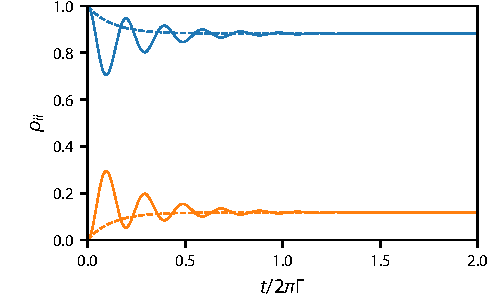
\includegraphics{figs/damped_rabi_flopping.pdf}
	\caption{\label{fig:rabi_flopping} Damped Rabi flopping for a two level atom with states $\ket{0}$ and $\ket{1}$ with corresponding density operators $\rho_{00}$ (blue) and $\rho_{11}$ (red) with both the OBEs (solid) and the rate equations (dashed).  The paramters of the calculation are $\Delta/\Gamma=-4$ and $s_0=20$.}
\end{figure}

Next, consider a slightly more complicated $F=2\rightarrow F=3$ atom illuminated by $\pi$ light, starting in a stretched state $m_F=-2$.  In this configuration, the lasers will optically pump the atoms into a stretched state with $\langle F_z \rangle = 0$, corresponding to equal populations between $\pm m_F$ with maximal population in $m_F=0$.  This pumping process is depicted in Fig.~\ref{fig:optical_pumping}, using a detuning $\Delta/\Gamma = -2.73$ and $s_0\approx 1.35$, parameters that match the parameters used for a similar simulation in Ungar, {\it et. al.}~\cite{Ungar1989}\footnote{Note that $s_0$ therein is defined with the detuning included.}.  Fig.~\ref{fig:optical_pumping} also shows the solution to rate equations, which are nearly identical except at early times.  Within the simulation contained within the simulation directory, 

\begin{figure}
	\center
	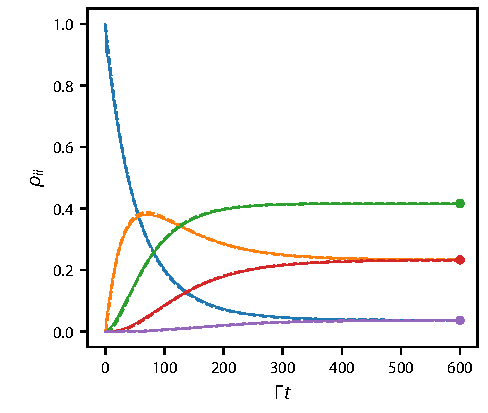
\includegraphics{figs/optical_pumping_f2_f3.pdf}
	\caption{\label{fig:optical_pumping} Optical pumping on an $F=2\rightarrow F'=3$ transition of an atom.  The populations of the $m_F=-2, 1, 0, 1, 2$ states are shown in blue, orange, green, red, and purple, respectively.  The solution from the rate equations (OBEs) are shown as dashed (solid) curves.  See text for other parameters.}
\end{figure}

\subsection{Electromagnetically induced transparency}
Beyond the two-level atom considered above, the three-level atom can produce a multitude of more complicated physical phenomenon.  Perhaps the most well known is electromagnetically inducted transparency.   Consider an three-level atom in the $\Lambda$ configuration, with ground state $\ket{g}$, intermediate meta-stable state $\ket{r}$, and excited state $\ket{e}$.  We assume that $\Omega_{ge} = \Braket{g|d\cdot E|e} \gg \Omega_{re} = \Braket{r|d\cdot E|e}$.   In this limit, if both lasers are resonant with their respective ground state  to excited state transition, the strong laser opens a transparency window in the otherwise absorptive transition [??].

\begin{figure}
	\center
	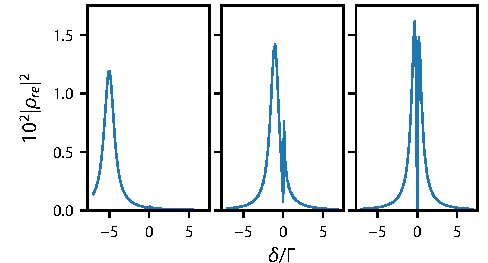
\includegraphics{figs/eit_susceptibility.pdf}
	\caption{\label{fig:eit_susceptibility} Susceptibility ($\rho_{re}$) of a three-level atom as a function of $\delta = \Delta_{ge}-\Delta_{re}$ for $\Delta_{ge}/\Gamma=-5$ (blue), $-1$ (orange), and $-0.1$ (green).}
\end{figure}

This effect is most easily seen by observing the susceptibility of the photons to the atom through the coherence $\rho_{re}$.  Figure~\ref{fig:eit_susceptibility} shows the numerically calculated $\rho_{re}$ for various values of $\delta/\Gamma = \Delta_{ge}/\Gamma-\Delta_{re}/\Gamma$, where $\Delta_{ie}$ is the detuning of the $i$th state laser from two-photon resonance with $\ket{e}$ for various $\Delta_{ge}$.  Here the parameters are $2(\Omega_{ge}/\Gamma)^2=10$ and $2(\Omega_{re}/\Gamma)^2=0.1$.  For $|\Delta_{ge}|\gg 1$, the absorption profile looks normal, except there is a small glitch in the susceptibility near Raman resonance at $\delta=0$.

\subsection{Two-level optical molasses}
While the previous examples focused exclusively on the internal structure of the atom, {\tt pylcp} is mostly focused on the coupling of the internal dynamics to the external motion.  Perhaps the most well-understood problem in this realm is the two-level atom moving in one dimension.

\begin{figure}
	\center
	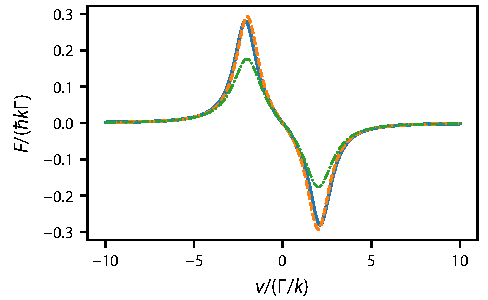
\includegraphics{figs/two_level_molasses_forces.pdf}
	\caption{\label{fig:two_level_molasses_forces} Force $F$ vs. velocity $v$ in a one-dimensional two-level molasses.  The three curves show the differences between the OBE (blue, solid), rate equations (orange, dashed), and heuristic equation (green, dashed).}
\end{figure}

The first step is to calculate the average force vs. velocity.  Fig.~\ref{fig:two_level_molasses_forces} shows such a force calculated using our three different governing equations for $\Delta/\Gamma=-2$ and $s_0=1.5$.  Equilibrium forces in an optical molasses are most accurately described using either the OBEs or the rate equations, which accurately account for saturation from the beams for all velocities.  The heuristic equation overestimates the saturation except near the origin, causing a reduction in force at $|v|\gg \Gamma/k$.  

\begin{figure}
	\center
	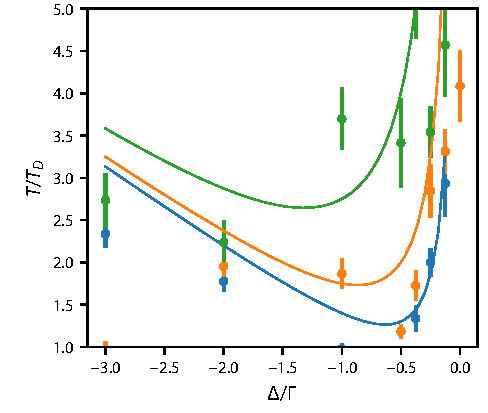
\includegraphics{figs/final_temperature_two_level_1D_molasses_rate_eqn.pdf}
	\caption{\label{fig:doppler_limit} Final temperature $T$ vs. detuning $\Delta$ and $s_0=0.3,\ 1,\ 3$ (blue, orange, green, respectively) for two-level atoms in a 1D molasses.  Error bars indicated 1-$\sigma$ uncertainty in the temperature.}
\end{figure}

Nevertheless, the damping force near the origin is nearly identical between the three equations when $\Delta/\Gamma$ is small.  This allows the results of two-level molasses~\cite{Lett1989} to be applicable to all three in such a regime.
Figure~\ref{fig:doppler_limit} shows the simulated temperatures of small clouds ($N=100$ atoms) simulated with the rate equations in such a 1D molasses.  We see reasonably good agreement with the expectation of Doppler cooling, Eq. (18) in Ref.~~\cite{Lett1989}.  Specifically, the solid curves show the expected value of 
\begin{equation}
	\label{eq:general_doppler_limit}
	\frac{T}{T_D} = \frac{1+2s_0+4(\Delta/\Gamma)^2}{4|\Delta/\Gamma|},
\end{equation}
where $T_D = \hbar \Gamma/2k_B$.  We note that in general we see a lower temperature than that predicted by \eqref{eq:general_doppler_limit} because 
the heuristic equation tends to underestimate the damping at larger detuning, and \eqref{eq:general_doppler_limit} comes from an analysis of the heuristic equation.

\subsection{Sub-Doppler molasses}
We can easily extend this study of one-dimenionsal molasses with more complicated level structures.  In particular, we focus on the $F=2\rightarrow F'=3$ transition in $^{23}$Na, which was studied first by Ungar, {\it et. al.}~\cite{Ungar1989}.  The calculate force profiles are shown in Fig.~\ref{fig:sub_doppler_force}.  This figure contains all of the essential features that were discussed in Ref.~\cite{Ungar1989}.  First, linear polarizations $\phi\neq=0$ and the so-called `corkscrew' polarization $\sigma^+\sigma^-$ produce sub-Doppler force features near zero velocity that are responsible for the additional damping.  Second, compared to the `two state' $\sigma^+\sigma^+$ polarization, $\sigma^+\sigma^-$ produces excess force due to the sub-Doppler discontinuty at $v=0$ that continues out to near $v/k\approx \Delta$, where one of the two lasers is dominantly resonant with the atom.  In the same example notebook, but omitted here, we also replicate the force's dependence on $s_0$ and detuning $\Delta$ observed in Ref.~\cite{Ungar1989}.

\begin{figure}
	\center
	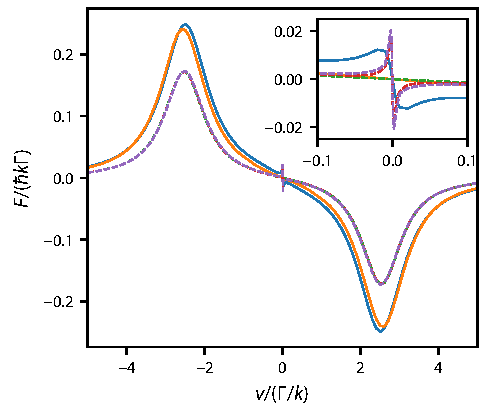
\includegraphics{figs/F2_to_F3_subDoppler_force}
	\caption{\label{fig:sub_doppler_force} Forces in a one-dimensional $F=2\rightarrow F'=3$ molasses with $\Delta/\Gamma=-2.5$ and $s_0=1.0$.  The solid curve correspond to circularly polarized beams: $\sigma^+\sigma^+$ (orange) and $\sigma^+\sigma^-$ (blue).  Dashed lines show linearly-polarized input beams with angles $\phi=0$ (green), $\phi=\pi/4$ (red), $\phi=\pi/2$ (purple). Inset shows features close to the origin.}
\end{figure}

%\begin{figure}
%	\center
%	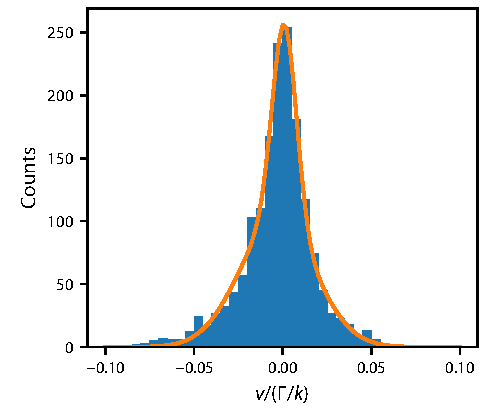
\includegraphics{figs/temperature_histogram_F2_to_F3}
%	\caption{\label{fig:sub_doppler_temperature} Sub-doppler temperature.}
%\end{figure}

In addition to the static force profiles, we also replicate the temperature observed via Monte-Carlo in Ref.~\cite{Ungar1989}.  In particular, we have simulated 96 atoms in the $\sigma^+\sigma^-$ configuration for a time $T=10^4/\Gamma$, and by sampling each atoms' velocity at a time interval $\delta t=500/\Gamma$ after allowing them to come into equilibrium with the light field for $2000/\Gamma$.  Fitting the resulting sampled velocities to a Gaussian reveals a temperature of  of $6.1(1.5)$~$\mu$K.  This temperature  compares nicely to the 8.2~$\mu$K obtained in Ref.~\cite{Ungar1989}.  We note that our temperature should be lower than that of Ref.~\cite{Ungar1989} as we do not include contributions to the momentum diffusion tensor from stimulated emission, for which they include an approximate contribution.

Contained in the examples directory, but omitted here, is a calculation of one-dimensional molasses for a variety of different polarizations and level structures, including those that utilize type-II transitions that have dark states.  Molasses operating on these transitions was studied in Ref.~\cite{Devlin2016} and the essential results are reproduced in the examples.

Another type of sub-Doppler molasses that is useful is that of three-level $\Lambda$-enhanced cooling~\cite{Grier2013}.  This molasses technique is unique compared to the others described above in that it uses a three-manifold system rather than a two-manifold.  We have simulated this process using {\tt pylcp}, and the script and results are contained with the other molasses examples.  The numerical results match the theoretical results of Ref.~\cite{Grier2013}.

\subsection{Force, capture, and temperature in MOTs}


Forces in a magneto-optical trap are slightly more complex than those of optical molasses, as they also depend on position as well as velocity.  Figure~\ref{fig:mot_forces} show such forces, calculated using the heuristic equation for such a one-dimensional MOT.  The laser parameters for this calculation are $\Delta/\Gamma=-1.5$ and $s_0=1$.  The white curves show trajectories, calculated without random scattering, of atoms injected into the MOT at a position $z=-20(\hbar \Gamma/\mu_B B')$ with varying initial velocity $v_0$.  Trajectories with $v_0 < 14\Gamma/k$ are captured, whereas trajectories with $v_0\geq 14 \Gamma/k$ escape.  ({\tt pylcp} contains routines to handle such bisection; no existing python package was found that does so.)  By calculating such trajectories and bisecting the initial velocity repeatedly, one can obtain the MOT capture velocity numerically.  Figure~\ref{fig:mot_forces} shows the result of such a calculation along with the prediction of a simple model found in Ref.~\cite{Haubrich1993}.  The two calculations agree rather well for small $s_0\leq 1$, but diverged by more than 10~\% for larger $s_0>1$.  This procedure has been extended to three-dimensional MOTs with non-standard geometry and should be the subject a forthcoming paper.

\begin{figure}
	\center
	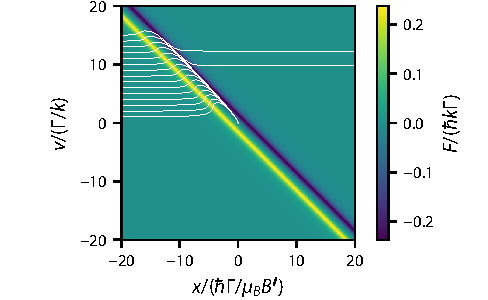
\includegraphics{figs/F0_to_F1_MOT_force_with_incoming_trajectories.pdf}
	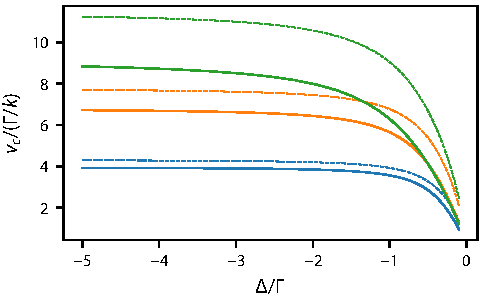
\includegraphics{figs/F0_to_F1_MOT_capture}
	\caption{\label{fig:mot_forces} (Top) Force $F$ vs. both position $x$ and velocity $v$ in a one-dimensional magneto-optical trap with laser parameters $\Delta/\Gamma=1.5$ and $s_0=1$.  The white curves show trajectories through phase space for atoms entering the MOT with different initial velocities $v_0$. (Bottom) Capture velocity $v_c$ vs. laser detuning $\Delta$ for $s_0=$ calculated using the heuristic equation for $s_0=0.3$ (blue), $1.0$ (orange), and $3.0$ (green).  Solid curves are the numerical results from {\tt pylcp}; dashed curves are the theoretical result from Ref.~\cite{Haubrich1993}.}
\end{figure}

This above example uses the heuristic equation, which calculates the textbook example of an $F=0\rightarrow F'=1$ atom.  Extending to larger $F$ and $F'$ in the one-dimensional case produces some intriguing results.  Consider Fig.~\ref{fig:mot_F1_to_F2} which shows an $F=1\rightarrow F'=2$ one-dimensional MOT with $g_F=0$ and $g_F'=1/F'$.  While not directly applicable to a specific atom, it is a good example of what occurs in alkaline earth atoms with nuclear spin, where the Lande g-factor in the ground state is $g_F\approx 0$.  Following the dashed line in Fig.~\ref{fig:mot_F1_to_F2}, which indicates the velocities/positions at which the rightward-going beam is resonant, we calculate the scattering rate for various transitions.  For $x<0$, the leftward going beam can become resonant, driving population from the cycling transition operating on $m_F=-1\rightarrow m_F'=-2$ into states with larger $m_F$.  For $x\ll \hbar\Gamma/\mu_B B'$, the atoms are mostly pumped into $m_F=+1$, wherem due to Clebsch-Gordon coefficients, they are significantly darker and therefore experience less force.  This curious effect is well known in narrow-line MOTs for alkaline earth atoms and requires a mixing laser to stir up population amongst the ground states of the atom in order to maintain optical cycling [??].

\begin{figure}
	\center
	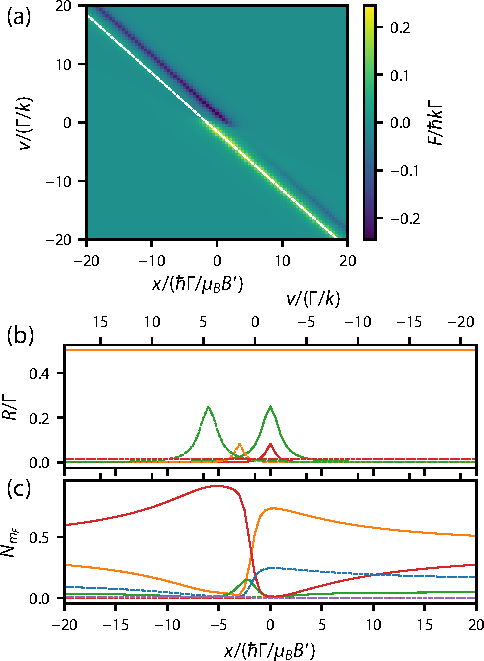
\includegraphics{figs/F1_to_F2_MOT_merged}
	\caption{\label{fig:mot_F1_to_F2} Anamoulous forces in a $F=1\rightarrow F'=2$ MOT with $g_F=0$ and $g_F'=1/F'$.  (a) Force $F$ vs. position $x$ and velocity $v$ for $\Delta/\Gamma=-4$ and $s_0=5$.  The dashed white line indicates the velocity/position combinations that are resonant with the laser beam traveling in the $+\hat{x}$ direction.  (b) Pumping rates from grond state $m_F=-1, 0, 1$ (orange, green, red, respectively) by the $+\hat{x}$ directed laser (solid) and the $-\hat{x}$ directed laser (dashed).  (c) Populations of the $m_F$ levels for ground (solid) and excited (dashed) states: $-2$ (blue), $-1$ (orange), $0$ (green), $1$ (red), $2$ (purple).}
\end{figure}

We also include an example calculation of the temperature of a $F=0\rightarrow F'=1$ magneto-optical trap, calculated in three dimensions with the optical Bloch equations.  Using $\Delta/\Gamma=-2.5$ and $s_0=1.25$ and simulated 96 atoms for $T=10^5/\Gamma$, sampling every $10^4/\Gamma$ for the latter half of the solution, we find a $T/T_D=3.9(1)$.  The example uses the default units described above and takes the mass of the atom simulated to be $\bar{m}=100$, closest to $^7$Li which has $\bar{m}\approx 46$.

\begin{figure*}
	\center
	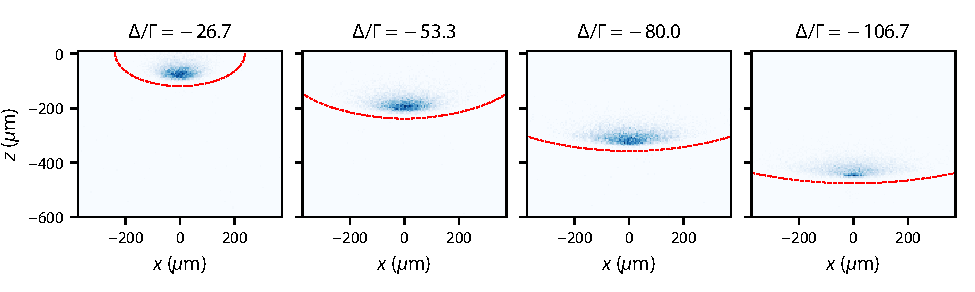
\includegraphics{figs/88Sr_red_MOT_differnt_detunings}
	\caption{\label{fig:recoil_limited_MOT} Simulated MOT images of the narrow line $^{88}$Sr MOT formed on the $^1 \mbox{S}_{0}\rightarrow ^3\mbox{P}_1$ transition for various detunings $\Delta$ and $s_0=25$.  Gravity is in the $-\hat{z}$ direction.  The red, dashed ellipses denote the spatial location where the beam detuning matches the Zeeman shift.  This figure should be compared to Ref.~\cite{Hanley2018}.}
\end{figure*}

Finally, we have also verified the calculation of Ref.~\cite{Hanley2018} of a recoil limited MOT.   Using the rate equations with random scattering and the parameters of $^{88}$Sr, we simulate the narrow-line MOT formed on the $^1 \mbox{S}_{0}\rightarrow ^3\mbox{P}_1$ transition.  The resulting images of the MOT with $N=1024$ atoms are shown in Fig.~\ref{fig:recoil_limited_MOT}.  One of the most unique features of this MOT is that it sags under the effect of gravity.  The vertical position and shape are mostly determined.  One effect we notice in our simulations that was not discussed in Ref.~\cite{Hanley2018} is atom loss.  We find that for $\Delta/\Gamma=-26.7$, we lose about 5~\% of the atoms from the MOT during a 50~ms simulation, and this increases with increasing detuning.  \SPE{Re-run to determine loss rate vs. detuning.} \SPE{Dan: consistent with experiment?}

Other MOT examples included with {\tt pylcp} include calculating MOT damping forces and trapping frequencies along with comparison to analytic formulas, the forces on both $D_1$ and $D_2$ lines of alkali atoms, the forces for a variety of different type-I and type-II MOTs considered in Ref.~\cite{Tarbutt2015}, and the forces in the two color CaF MOT of Ref.~\cite{Tarbutt2015a}. 

\subsection{Bi-chromatic forces}

\begin{figure}
	\center
	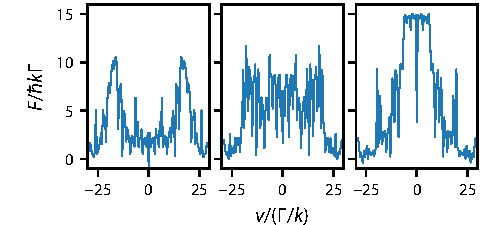
\includegraphics{figs/bichromatic_force}
	\caption{\label{fig:bichromatic} Force vs. velocity for a two-level atom in an intense bi-chromatic standing wave for $\Delta/\Gamma=39$.  The intensities are $\Omega =39\Gamma$ (left), $\Omega =43\Gamma$ (middle), and $\Omega =47\Gamma$ (right), as in Fig.~1 of Ref.~\cite{Soding1997}.}
\end{figure}

One can also calculate forces due to stimulated emission, unlike all the examples prior which relied solely on spontaneous emission.  A common setup for stimulated optical forces is the bichromatic force, which involves creating counterpropogating $\pi$ pulse trains to excite the atom to the excited state from one direction and stimulate it back down to the ground state via $\pi$ pulses from the opposite direction.  This stimulated optical force was examined theoretically and demonstrated experimentally in Ref.~\cite{Soding1997}.   Here, the pulses were made by shining two frequencies of light from both directions, each frequency detuned by $\pm\Delta$.  The necessary phases between all four frequencies must be well established to ensure the direction of stimulated emission is proper.  Fig.~\ref{fig:bichromatic} shows the calculation of the force for a two-level atom in this laser arrangement using {\tt pylcp}.  For each intensity, the force exceeds the spontaneous force limit of $\hbar k \Gamma$, and has a host of curious features including Doppleron resonances.  By simulating these in {\tt pylcp}, one can easily extend this to more complicated systems such as real atoms or molecules, and examine how operating bi-chromatic forces on non-cycling transitions may impact the size of the resulting forces.

\section{Conclusion}
We have presented 
%% The Appendices part is started with the command \appendix;
%% appendix sections are then done as normal sections
%% \appendix

%% \section{}
%% \label{}

%% References
%%
%% Following citation commands can be used in the body text:
%% Usage of \cite is as follows:
%%   \cite{key}         ==>>  [#]
%%   \cite[chap. 2]{key} ==>> [#, chap. 2]
%%

%% References with bibTeX database:

\bibliographystyle{elsarticle-num}
\bibliography{pylcp}

%% Authors are advised to submit their bibtex database files. They are
%% requested to list a bibtex style file in the manuscript if they do
%% not want to use elsarticle-num.bst.

%% References without bibTeX database:

% \begin{thebibliography}{00}

%% \bibitem must have the following form:
%%   \bibitem{key}...
%%

% \bibitem{}

% \end{thebibliography}


\end{document}

%%
%% End of file
